% vim: set tw=78 sts=2 sw=2 ts=8 aw et ai:
\subsection{Opportunistic Linked Increases Algorithm - OLIA}
OLIA (Opportunistic Linked Increases Algorithm) is the current default congestion control algorithm used by MPTCP. It is the successor of LIA (Linked Increases Algorithm), having been developed to address LIA's performance issues, namely its lack of pareto-optimality. OLIA is a window-based congestion control algorithm which couples the increase of congestion windows and uses unmodified behavior in case of a loss \cite{olia}.

OLIA increases the congestion window for each subflow on each ACK received on that subflow based on RTTs and the congestion windows of all the subflows available to the user. The algorithm guarantees both responsiveness and non-flappiness while removing the tradeoff between responsiveness and optimal load balancing which plagued LIA. OLIA is proven to satisfy the goals of a good multipath congestion control algorithm: improve throughput, do no harm and balance congestion \cite{olia}.

\subsection{Weighted Vegas - wVegas}
Weighted Vegas (wVegas) is a delay-based congestion control algorithm for MPTCP which achieves fine-grained load balancing by using packet queuing delay as a congestion signal \cite{wvegas}. Linked Increases algorithms such as LIA and OLIA use packet loss as a sign of congestion and will only shift packets between paths after the loss event has been detected. In practice, they are reactive algorithms and only provide an estimation of the extent of congestion. The creators of wVegas argue that traffic should be shifted as early as possible, before losses occur. Therefore they propose an approach based on what they define as the Congestion Equality Principle: "if every flow strives to equalize the extent of congestion that it perceives on all its available paths by means of shifting traffic, then network resources will be fairly and efficiently shared by all the flows" \cite{wvegas}.

The implementation of wVegas is based on TCP-Vegas. During the congestion avoidance phase, the congestion window is increased or decreased based on the average RTT in the previous round of congestion avoidance and the minimal RTT recorded so far. The subflow weight adjustment algorithm of wVegas manages to achieve good convergence and timely traffic shifting \cite{wvegas}.

\subsection{Improved Testbed}
The amount of virtualization in our previous testbed incurred significant overhead which we believe affected performance. We used a Ubuntu 12.04 virtual machine with software defined networking framework Mininet. Inside Mininet we defined two hosts with an Ethernet link between them. OpenVPN tunnels were created over the link. While Mininet offered useful features for link control and topology definition, the additional layer created by its process-based virtualization proved problematic.

For this stage we have completely revamped our testing environment, outlined
in Figure \ref{fig:testbed}. It now
consists of two separate Ubuntu 14.04 virtual machines with OpenVPN tunnels
running on the single link between them. The virtualization technology is KVM,
which offers improved performance and reduced overhead. Setup scripts run on
both machines, creating the necessary interfaces and OpenVPN tunnels and
configuring system parameters, network parameters and link bandwidth and delay
limitations. The previous performance penalty induced by the Mininet
framework is no longer of concern.

\begin{figure}[H]
  \centering
  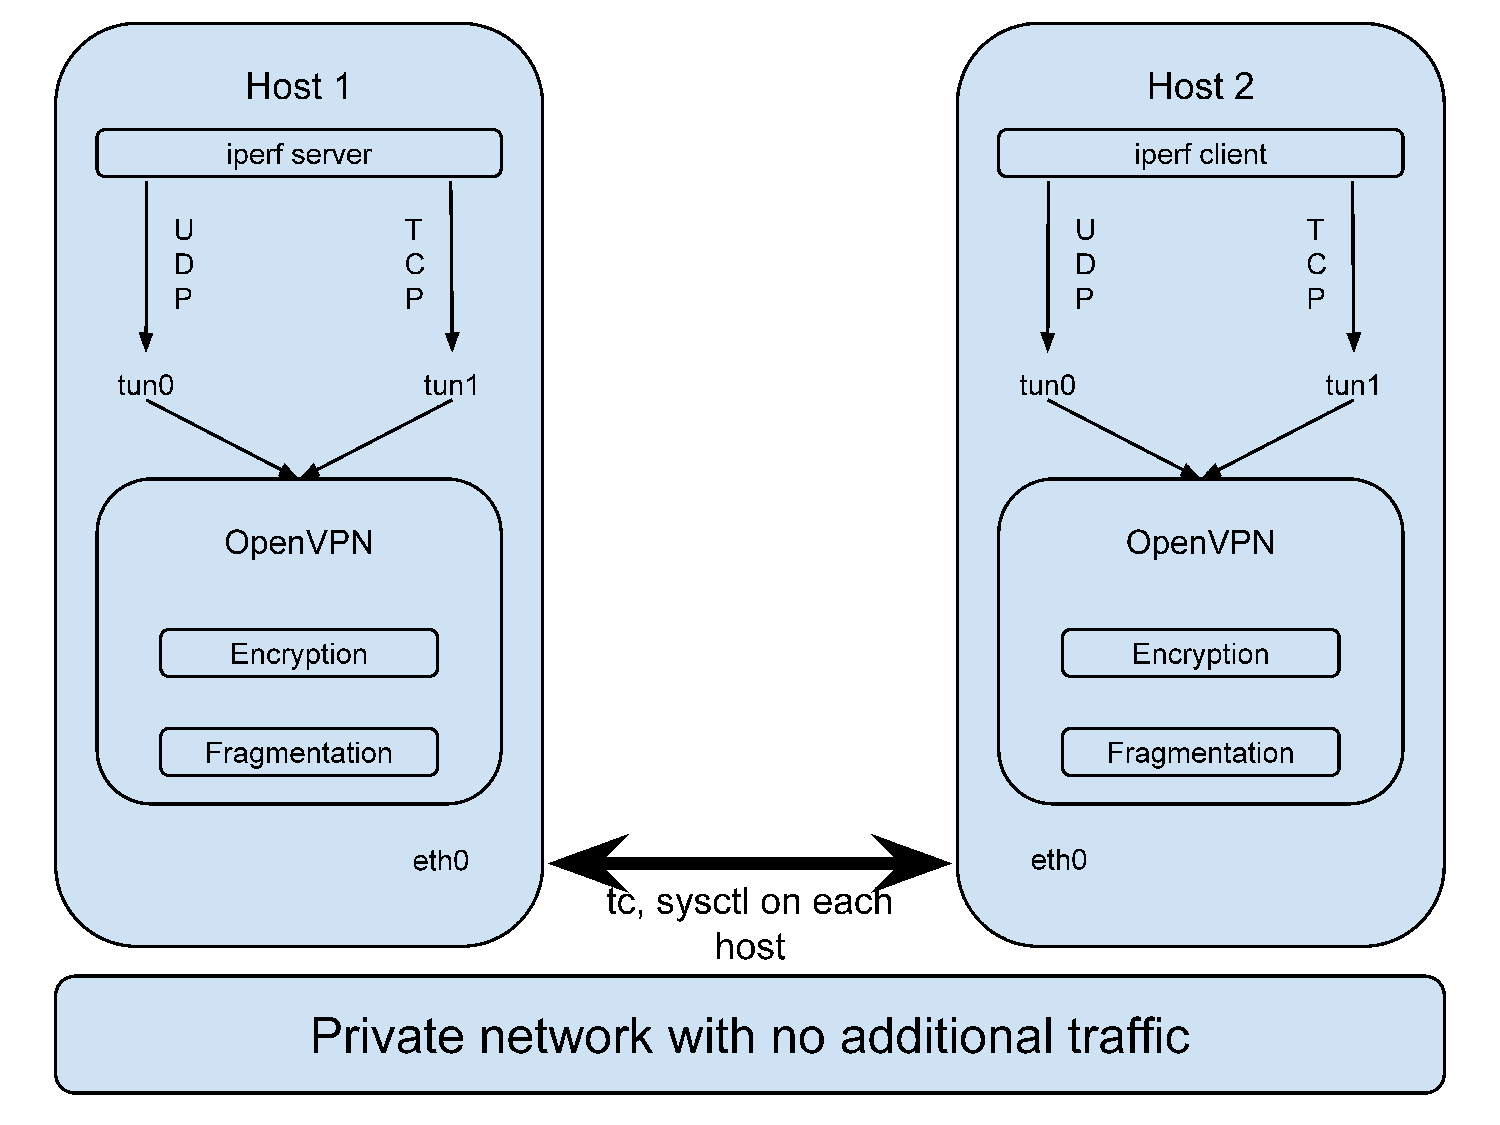
\includegraphics[width=0.5\textwidth]{img/mptcp-openvpn-bare}
  \caption{New MPTCP testbed}
  \label{fig:testbed}
\end{figure}

Our previous environment also suffered from constraints which prevented us from configuring different bandwidth and delay values for each tunnel over the Ethernet link. As a consequence, all our tests assumed the conditions for all tunnels were the same. In the real world, one of the usecases for link aggregation is represented by mobile devices which have at least two different network interfaces, WiFi and 3G. Since WiFi and 3G are very different in terms of bandwidth but especially delay, we need to be able to configure different link conditions in our experiments. This feature was added to the current version of the software.

The other system and link configuration methods have remained largely the
same. Despite reducing the computational overhead we still eliminate
encryption and message authentication. We use the sysctl interface of the
Linux kernel to modify TCP and UDP buffer sizes. We deactivate inet peer
storage and clear the route cache after every test. With regards to OpenVPN,
we control the send and receive buffers, the MTU and we deactivate its
internal fragmentation engine.
